\documentclass{standalone}
\usepackage{tikz}
\usepackage{amsmath}
\usetikzlibrary{bayesnet}

% Provides the following node styles:

%     latent
%     obs
%     det
%     const
%     factor
%     plate
%     gate

% Provides the following commands (note that any of the arguments can be empty):

%     \factor [options] {name} {caption} {inputs} {outputs}
%     \plate [options] {name} {fitlist} {caption}
%     \gate [options] {name} {fitlist} {inputs}
%     \vgate {name} {fitlist-left} {caption-left} {fitlist-right} {caption-right} {inputs}
%     \hgate {name} {fitlist-top} {caption-top} {fitlist-bottom} {caption-bottom} {inputs}
%     \edge [options] {inputs} {outputs}
%     \factoredge [options] {inputs} {factors} {outputs}
\begin{document}
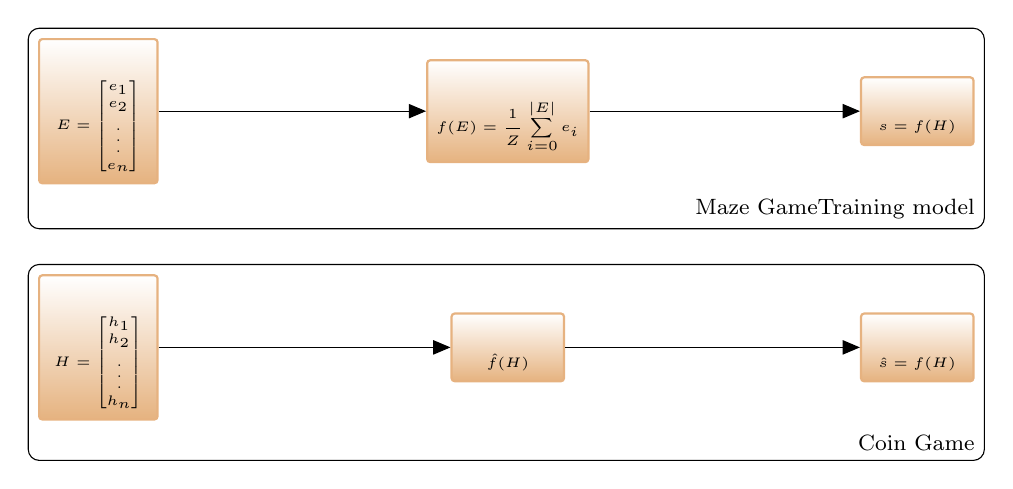
\begin{tikzpicture}[
    node distance=2mm,
    title/.style={font=\fontsize{6}{6}\color{black!50}\ttfamily},
    typetag/.style={rectangle, minimum size=1mm, rounded corners=0.4mm, thick, draw=orange!80!black!50, top color=white, bottom color=orange!80!black!50, font=\tiny},
    typetag1/.style={rectangle, minimum size=10mm, rounded corners=1mm, thick, draw=orange!80!black!50, top color=white, bottom color=orange!80!black!50, font=\tiny}
    ]
    \node (ein) [typetag, xshift=74mm, yshift=0mm]  {
      \begin{minipage}{.5in}
        \centering
          \begin{align*}
          E &= 
          \begin{bmatrix}
             e_{1} \\
             e_{2} \\
             \vdots \\
             e_{n}
          \end{bmatrix}
        \end{align*}
      \end{minipage}  
    };
    \node (fe) [typetag, right of=ein, xshift=+50mm]  {
      \begin{minipage}{.47in}
        \centering
          \begin{align*}
          f(E) &=
          \frac{1}{Z}\sum_{i=0}^{|E|} e_i
        \end{align*}
      \end{minipage}  
    };

    \node (eout) [typetag, right of=fe, xshift=+50mm]  {
      \begin{minipage}{.47in}
        \centering
          \begin{align*}
          s = f(H)
        \end{align*}
      \end{minipage}  
    };

    \edge {ein} {fe}
    \edge {fe} {eout}
    \plate {maze_game} {(ein)(fe)(eout)} {Maze Game\\ Training model}
    \node (hin) [typetag, xshift=74mm, yshift=-3cm]  {
      \begin{minipage}{.5in}
        \centering
          \begin{align*}
          H &= 
          \begin{bmatrix}
             h_{1} \\
             h_{2} \\
             \vdots \\
             h_{n}
          \end{bmatrix}
        \end{align*}
      \end{minipage}  
    };
    \node (fh) [typetag, right of=hin, xshift=+50mm]  {
      \begin{minipage}{.47in}
        \centering
          \begin{align*}
          \hat{f}(H)
        \end{align*}
      \end{minipage}  
    };

    \node (hout) [typetag, right of=fh, xshift=+50mm]  {
      \begin{minipage}{.47in}
        \centering
          \begin{align*}
          \hat{s} = f(H)
        \end{align*}
      \end{minipage}  
    };

    \edge {hin} {fh};
    \edge {fh} {hout};
    \plate {coin_game} {(hin)(fh)(hout)} {Coin Game};
\end{tikzpicture}
\end{document}